%%\title{APERTURE AND TOLERANCES}
%  Changed by: Mark HAYES, 19-Sep-2002 
%  Changed by: Ivar Waarum, 24-Feb-2005 
 
\chapter{Physical Aperture}
\label{chap:aperture}

Physical apertures can be defined and associated to most elements 
in \madx. 
 
The \hyperref[sec:aperture]{\texttt{APERTURE}} command calculates 
the beam stay clear values (n1 values). 

During tracking the particle excursion can be checked against the 
available aperture, and the particle lost if it falls outside 
the defined aperture.


\section{Aperture definition}
\label{sec:def-aper}
The aperture for a particular element or class of elements can be 
set in \madx at the time of definition or instantiation of the 
element or class. 

Note that instantiation can also happen at the time of declaration of 
an element in a \hyperref[chap:sequence]{sequence}.  

The aperture can be specified for any element or class of elements, 
with the exception of drift spaces. 

The definition of the aperture takes the following form and parameters:\\
\madbox{
 ..., \=APERTYPE=string,  APERTURE=\{values\}, \\
      \>APER\_OFFSET=\{values\}, APER\_TOL=\{values\},...
}

where the four specific  attributes are attributes of an element 
declaration or instantiation. 

The minimum aperture definition uses the following two attributes:

%% A new feature of MAD-X is the ability to set an aperture for a
%% particular  element, or parent of a set of elements. This removes the
%% need of placing a collimator next to every element to do aperture
%% tracking.  The aperture of any elements can be specified (excepts
%% drifts) by the use of the following parameters:  



\begin{madlist}
  \ttitem{APERTYPE} defines the aperture type from a set of
  preselected types, or from a file if a filename is provided as argument.
  The preselected types are:
  \begin{madlist}
    \ttitem{CIRCLE}
    \ttitem{RECTANGLE} 
    \ttitem{ELLIPSE} 
    \ttitem{RECTCIRCLE} a superposition of a \texttt{CIRCLE} and a
    \texttt{RECTANGLE}  
    \ttitem{LHCSCREEN} an alias for \texttt{RECTCIRCLE}
    \ttitem{RECTELLIPSE} a superposition or intersection of an
    \texttt{ELLIPSE} and a \texttt{RECTANGLE} 
    \ttitem{RACETRACK} the union of an \texttt{ELLIPSE} and a 
    \texttt{RECTANGLE} forming a \texttt{RACETRACK} shape with four
    quarters of ellipse, one per quadrant, connected by straight lines
    \ttitem{OCTAGON} a simply connex octagon
  \end{madlist}
  If a filename is provided as argument, the file must contain a 
  list of x and y coordinates, one pair per line, outlining the complete aperture shape, 
  i.e. no symmetry is assumed. This option is only supported by the 
  \hyperref[chap:aperture]{\texttt{APERTURE}} module and an aperture thus defined is 
  ignored in the \hyperref[chap:thintrack]{\texttt{TRACK}} module.
  When a filename is provided as argument, the \texttt{APERTURE} attribute is ignored.\\
  \\
  \ttitem{APERTURE} is an array of values, the number and meaning 
  of which depends on the \texttt{APERTYPE}.  
\end{madlist}

\begin{table}[ht]
  \caption{Predefined aperture types}
  \label{table:apertype}
  \vspace{1ex}
  \begin{tabular}{|l | c | p{7.5cm}|}
    \hline 
    \textbf{APERTYPE} & \textbf{\# of values} & \textbf{meaning of values}\\
    \hline
    \texttt{CIRCLE} & 1 &  radius of circle \\
    \hline
    \texttt{RECTANGLE} & 2 & half width and half height of rectangle\\ 
    \hline
    \texttt{ELLIPSE} & 2 & horizontal and vertical semi-axes of ellipse \\  
    \hline
    \texttt{RECTCIRCLE} or \texttt{LHCSCREEN} & 3 & half width and half height 
    of rectangle, radius of circle\\
    \hline
    \texttt{RECTELLIPSE} & 4 & half width and half height of rectangle, 
    horizontal and vertical semi-axes of ellipse \\
    \hline
    \texttt{RACETRACK} & 4 & half width and half height along main axes, 
    and horizontal and vertical semi-axes of ellipse for the rounding 
    of the corners \\
    \hline
    \texttt{OCTAGON} & 4 & half width and half height along main axes, 
    two angles sustaining the cut corner in the first quadrant, 
    given in radians and in order of increasing values. \\   
    \hline
  \end{tabular}
\end{table}

\vskip 5mm

\textbf{Examples}\\
The following statements are equivalent in setting an elliptic aperture 
using the variables \texttt{APH} and \texttt{APV}:
\madxmp{
..., APERTYPE=ellipse, APERTURE=\{APH, APV\}; \\
..., APERTYPE=rectellipse, APERTURE=\{APH, APV, APH, APV\}; \\
..., APERTYPE=racetrack, APERTURE=\{APH, APV, APH, APV\}; 
}

Similarly the following statements are equivalent in setting a rectangular 
aperture using the variables \texttt{APX} and \texttt{APY}, 
and \texttt{APR:=SQRT(APX**2+APY**2)}:
\madxmp{
..., APERTYPE=rectangle, APERTURE=\{APX,APY\}; \\
..., APERTYPE=rectellipse, APERTURE=\{APX, APY, APR, APR\}; \\
..., APERTYPE=racetrack, APERTURE=\{APX, APY, 0.0, 0.0\}; 
}

When the aperture is described in a file, the only parameter to be provided is 
a filename given as value to the \texttt{APERTYPE} attribute:
\madxmp{
MB: SBEND, L=l.MB, APERTYPE="MB-aper.txt";
}
where \texttt{"MB-aper.txt"} contains the list of x-y coordinates defining the
aperture shape:
\madxmp{
*****\= \kill
x0   \>y0 \\
xi   \>yi \\
\ldots \\
xn   \>yn
}

\textbf{Notes}
\begin{itemize}
   \item There are inconsistencies in the parameter definition for the
     different aperture types. This is historical and is kept for
     backwards compatibility. Pay some attention to the parameters you
     introduce! 


	\item The \texttt{RECTELLIPSE}  and \texttt{RACETRACK} shapes are fundamental 
	in the sense that both can properly model the other \texttt{CIRCLE}, 
	\texttt{ELLIPSE} and \texttt{RECTANGLE} shapes, and that \texttt{RECTCIRCLE} 
	and \texttt{LHCSCREEN} shapes are a particular of \texttt{RECTELLIPSE}

	\item It is considered good practice to always set the first two 
	\texttt{APERTURE} parameters for predefined shapes to be the maximum
	horizontal and vertical extents. This proves useful when trying to 
	plot horizontal and vertical beam stay-clear. 
	For example, it is better to use
	\madxmp{
..., APERTYPE=rectellipse, APERTURE={APX, APY, APX, APY};
	}
	rather than
	\madxmp{
..., APERTYPE=rectellipse, APERTURE={100, 100, APX, APY};
	}

   \item When \hyperref[chap:makethin]{\texttt{MAKETHIN}} is called all
     thin slices inherit the aperture of their respective original thick
     lens version.  

   \item When the \hyperref[chap:sixtrack]{\texttt{SIXTRACK}} command is called (see the
     \hyperref[chap:sixtrack]{SixTrack converter module}) the apertures are
     ignored by default. To convert the apertures as well the \texttt{APERTURE}
     flag has to be set in \texttt{C6T}.  

   \item  Aperture parameters are like all parameters and are inherited
     by derived elements. Like other parameters they can also be overridden by
     the derived elements if necessary.  

   \item The \texttt{APERTYPE} and the \texttt{APERTURE}s themselves can be
     conveniently added to the \hyperref[chap:twiss]{\texttt{TWISS}} 
     (\autoref{chap:twiss}) table by using the
     \hyperref[sec:select]{\texttt{SELECT}} command
     (\autoref{sec:select}). For example the command:     
\madxmp{
xxxxxxxxxxxxxxxxxxxxxxxxxxx\= \kill
Select, flag=twiss, clear; \\
Select, flag=twiss, column= \>name,s,betx,alfx,mux,bety,alfy,muy, \\
                            \>apertype,aper\_1,aper\_2; \\
}
     and a subsequent \texttt{TWISS} command put the aperture information together 
     with the specified \texttt{TWISS} parameters into the \texttt{TWISS} table.

   \item The minimum beam stay-clear value (n1 value) computed along the 
     beamline is printed to standard out and is also available as an output 
     variable \texttt{N1MIN} of the \hyperref[sec:beam]{\texttt{BEAM}} command: 
\madxmp{
Value, beam->n1min;\\
nmin = beam->n1min;
}

\end{itemize}

\section{Aperture tolerance definition}
\label{sec:apertol}
A parameter closely connected to the aperture is the sum of the
mechanical and alignment tolerances. The mechanical tolerance is 
the maximal error margin of errors in the element body which 
causes a decrease of aperture, and the alignment tolerance is a 
misalignment of the element in the accelerator, which also causes a 
decrease of aperture. The tolerance is given in the transverse plane 
as a racetrack, like in picture \ref{fig:aperture-tol} below. 

\begin{figure}[htb]
  \centering
  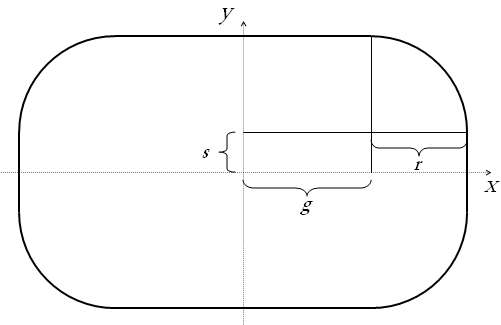
\includegraphics[width=250bp]{jpg/tolerance.jpg}
  \caption{Definition of aperture tolerances}
  \label{fig:aperture-tol}
\end{figure}

A tolerance can be assigned to each element in a \madx sequence as a vector: 
\madbox{
APER\_TOL = \{r, g, s\};
}
\textbf{Example:}
\madxmp{
MB: SBEND, L=l.MB, APER\_TOL=\{1.5, 1.1, 0\};
}

\section{Aperture offset definition}
\label{sec:aperoffset}

An aperture offset can be assigned to each element in a \madx sequence as a vector: 
\madbox{
APER\_OFFSET = \{real, real\};
}

where the two real values are respectively the horizontal and vertical
offsets of the aperture inside the element. 

The offsets are only used in the
\hyperref[chap:thintrack]{\texttt{tracking}}  
module of \madx and are ignored by the \texttt{APERTURE} command and by 
\hyperref[sec:ptc-track]{\texttt{PTC\_TRACK}}.


\section{APERTURE}
\label{sec:aperture}
\textbf{The APERTURE module was developed specifically for the LHC.\\ 
Default parameter values are LHC values.} 

The \texttt{APERTURE} module computes the \texttt{n1} values for a piece of machine. 
Each element is sliced into thick sub-elements at given intervals, and
the available aperture is computed at the end of each slice. 
The \texttt{APERTURE} module gets the geometric emittances from the values given 
or calculated in the \hyperref[chap:beam]{\texttt{BEAM}} command. 
The computation is based on the last Twiss table computed by the 
\hyperref[chap:twiss]{\texttt{TWISS}} command. 
It is important to properly define a \texttt{BEAM}, and run 
\hyperref[chap:twiss]{\texttt{TWISS}} and \texttt{APERTURE} commands 
on the same period or sequence.

The \texttt{APERTURE} example below also shows how to \hyperref[chap:plot]{plot} 
the resulting \texttt{n1} values.

The minimum \texttt{n1} value is written to the last Twiss table, to
allow for \hyperref[chap:match]{matching by aperture}.

\madbox{
APERTURE, \=RANGE=range, \\
          \>DQF=real, DPARX=real, DPARY=real, \\
          \>BETAQFX=real, BBEAT=real, DP=real, \\
          \>COR=real,  NCO=integer, \\
          \>HALO=\{real,real,real,real\}, HALOFILE=filename,\\
          \>INTERVAL=real, SPEC=real, NOTSIMPLE=logical, \\
          \>TRUEPROFILE=filename, OFFSETELEM=filename, \\
          \>FILE=filename;  
}

where the parameters have the following meaning: 
\begin{madlist}
	\ttitem{RANGE} \hyperref[sec:range]{Range} given by
	elements. Default = \texttt{\#s/\#e}  
	\ttitem{DQF} Peak linear dispersion [m]. Default = 2.086 
	\ttitem{DPARX} Fractional horizontal parasitic dispersion. Default = 0.273 
	\ttitem{DPARY} Fractional vertical parasitic dispersion. Default = 0.273 
	\ttitem{BETAQFX} Beta x in standard qf [m]. Default = 170.25 
	\ttitem{BBEAT} Beta beating coefficient applying to beam size. Default = 1.1 
	\ttitem{DP} Bucket edge at the current beam energy. Default = 0.0015 
	\ttitem{COR} Maximum radial closed orbit uncertainty [m]. Default = 0.004 
	\ttitem{NCO} Number of azimuth per quadrant for halo radial scan. Default = 5 
	\ttitem{HALO} Halo parameters: \{n, r, h, v\}. n is the radius of the
	primary halo,  r is the radial part of the secondary halo, h and v
	is the horizontal and  vertical cuts in the secondary halo. Default
	= \{6, 8.4, 7.3, 7.3\}  
	\ttitem{HALOFILE} Input file with halo polygon coordinates. Will
	suppress  an eventual halo parameter. Default = none  
	\ttitem{INTERVAL} Approximate length in meters between
	measurements. Actual value:  nslice = nodelength/interval, nslice
	is rounded down to closest integer,  interval =
	nodelength/nslice. Default = 1.0  
	\ttitem{SPEC} Aperture spec, for plotting only. Gives the spec line in
	the plot. Default = 0.0  
	\ttitem{NOTSIMPLE} Use only if one or more beam-screens in the range are
	considered not to  be a "simply connex". Since all predefined \madx aperture 
	types are simply connex, this is only possible  if an input file with
	beam screen coordinates are given. See below for a graphical
	example. Default = false.  
	\ttitem{TRUEPROFILE} A file containing a list of magnets, and for each
	magnet a list of horizontal and vertical deviations from the ideal
	magnet axis. These values may come from measurements done on the
	magnet. See below for example. Default = none.  
	\ttitem{OFFSETELEM} A file containing a reference point in the machine,
	and a list of magnets with their offsets from this point described
	as a parabola. See below for example. Default = none. \\
	\textbf{Note that the reference point should be within the range of
	elements given for the offsets to be taken into account.}
	\ttitem{FILE} Output file with aperture table. Default = none 
\end{madlist}

\section{Not simply connex beam pipe profiles} 
\label{sec:notconnex}
The algorithm for finding the largest possible halo is the following: \\
The distance from halo centre to the first apex (i = 0)
in the halo is calculated (l\_i), and the equation for a line going
through these points is derived. This line is then compared with all
lines making the pipe polygon to find their respective intersection
coordinates. The distance h\_i between halo centre and intersection are
then divided by l\_i, to find the maximal ratio of enlargement, as seen
in figure \ref{fig:notsimple0} below. 
This procedure is then repeated for all apexes i in the halo
polygon, and the smallest ratio  of all apexes is the maximal
enlargement ratio for this halo to just touch the pipe at this
particular longitudinal position. 

\begin{figure}[h]
  \centering
  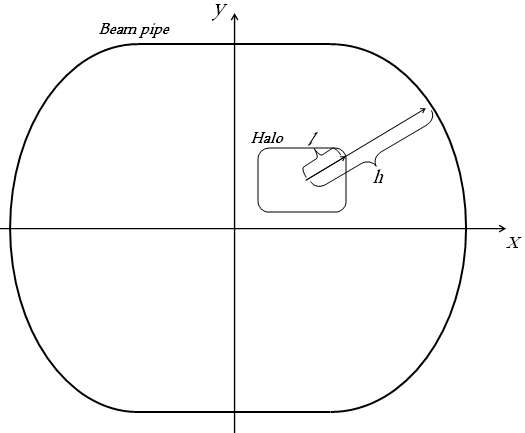
\includegraphics[width=250bp]{jpg/notsimple0.jpg}
  \caption{Determination of maximum halo size}
  \label{fig:notsimple0}
\end{figure}

There is one complication to this solution; polygons which are not
simple connexes. (Geometrical definition of ``simply connex'': A figure
in which any two points can be connected by a line segment, with all
points on the segment inside the figure.) The figure \ref{fig:notsimple1}
below shows what happens when a beam pipe polygon is not a simple
connex. The halo is expanded in such a way that it overlaps the external
polygon in the area where the latter is dented inwards. 

\begin{figure}[htb]
  \centering
  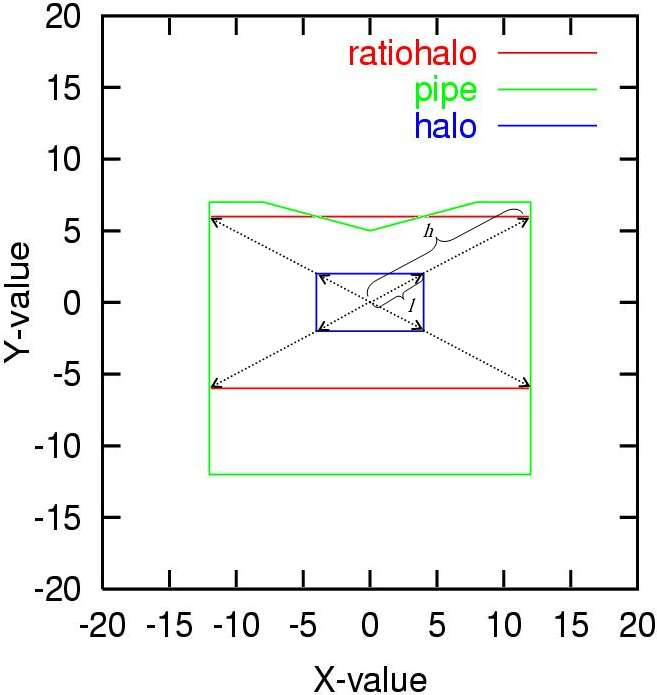
\includegraphics[width=250bp]{jpg/notsimple1.jpg}
  \caption{Not connex beam pipe profile: problem}
  \label{fig:notsimple1}
\end{figure}

\begin{figure}[htb]
  \centering
  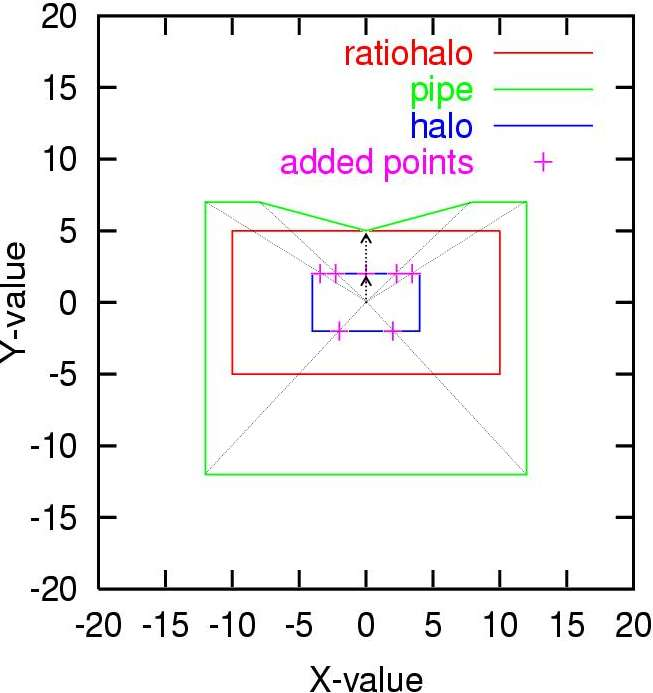
\includegraphics[width=250bp]{jpg/notsimple2.jpg}    
  \caption{Not connex beam pipe profile: solution}
  \label{fig:notsimple2}
\end{figure}

To make the module able to treat all sorts of polygons, the logical
attribute \texttt{NOTSIMPLE} must be specified. With this option activated,
apexes are strategically added to the halo polygon wherever the beam pipe
polygon might have an inward dent. This is done by drawing a line from
halo centre to each apex on the pipe polygon. An apex with its
coordinates on the intersection point line-halo is added to a table of
halo polygon apexes. The result is that the halo polygon has a few
``excessive'' points on straight sections, but the algorithm used for
expansion will henceforth not miss a dent in the beam pipe. See
figure \ref{fig:notsimple2}. The use of the
notsimple option significantly increases computation time. 

\section{Trueprofile file syntax}
\label{sec:trueprofile}
This file contains magnet names, and their associated displacements of
the axis for  an arbitrary number of S, where So is the start of the
magnet and Sn the end. The interval between each S must be regular, and
X and Y  must be given in meters. The magnet name must be identical to
how it appears in the  sequence. The displacements are only valid for
this particular magnet, and cannot be  assigned to a family of
magnets. n1 is calculated for a number of slices determinated by the
number of Si. 
\\
\textbf{Layout of file:}
\madxmp{
xxxxx\=xxx\= \kill
magnet.name1 \\
So   \>X   \>Y \\
Si   \>X   \>Y \\
Si   \>X   \>Y \\
Sn   \>X   \>Y \\
\\
magnet.name2 \\
So   \>X   \>Y \\
Si   \>X   \>Y \\
Si   \>X   \>Y \\
Sn   \>X   \>Y \\
\\ 
etc.
}

\textbf{Example of file:}
\begin{verbatim}
mb.a14r1.b1
0        0.0002        0.000004
7.15     1.4e-5        0.3e-3
14.3     0.0000000032  4e-6

mq.22r1.b1
0      0.3e-5     1.332e-4
1.033  0.00034    0.3e-9
2.066  0          0.00e-2
3.1    4.232e-4   0.00000003
\end{verbatim}

\section{Offsetelem file syntax}
\label{sec:offsetelem}
This file contains parameters describing how certain elements are
actually located in space with respect to a given reference element in
the machine.  

The basis for this file is a pair of coordinate systems, \{s,x\} and \{s,y\} 
with the origin at the reference point. The units for s, x and y are
meters.

The actual location of the magnetic axis of a given element can be
described, in each plane, as a parabola defined with three coefficients: 
\madxmp{
X\_act(s) = DDX\_OFF * s**2  +  DX\_OFF * s  +  X\_OFF \\
Y\_act(s) = DDY\_OFF * s**2  +  DY\_OFF * s  +  Y\_OFF
}

The reference position for the element, X\_ref(s) and Y\_ref(s), is
calculated  by \madx via an internal call to the
\hyperref[chap:survey]{\texttt{SURVEY}} module, taking the reference element
as the origin.   

The resulting offset, in each plane, which is taken into account in the
aperture calculation, is the difference between reference position and
actual position:  
\madxmp{
X\_offset(s) = X\_ref(s) - X\_act(s) \\
Y\_offset(s) = Y\_ref(s) - Y\_act(s)
}

The offsets are only calculated for elements for which actual positions 
have been given through the \texttt{OFFSETELEM} file mechanism. 

The file must be given in \texttt{TFS} format according to the following
template, with mandatory header and any number of data lines, one per element. 

{\footnotesize
\begin{verbatim}
@ NAME             %06s "OFFSET" 
@ TYPE             %06s "OFFSET" 
@ REFERENCE        %10s "reference-element-name" 
* NAME          S_IP       X_OFF     DX_OFF    DDX_OFF    Y_OFF    DY_OFF     DDY_OFF
$ %s            %le        %le       %le       %le        %le      %le        %le
"elementname"   real       real      real      real       real     real       real
\end{verbatim}}

Note that the column \texttt{S\_IP} is actually not used, and the values
are ignored, but the column and values are parsed nevertheless and must
be present. The absence of this column will trigger an error. 

\textbf{Example:}
{\footnotesize
\begin{verbatim}
@ NAME             %06s "OFFSET" 
@ TYPE             %06s "OFFSET" 
@ REFERENCE        %10s "mq.12r1.b1" 
* NAME          S_IP       X_OFF     DX_OFF    DDX_OFF    Y_OFF    DY_OFF     DDY_OFF
$ %s            %le        %le       %le       %le        %le      %le        %le
"mq.12r1.b1"    0.0        -3.0      -2.56545   0.0       0.0      -2.344366  0.0
"mcbxa.3r2"     0.0        -0.84     32.443355  0.3323    0.0      32.554363  0.2522
\end{verbatim}}

%A python script to convert a file from the old V.3.XX format to the new V4.xx can be found at :
%/afs/cern.ch/eng/lhc/optics/V6.503/aperture/convert_offsets.py
%usage : convert_offsets.py filename

As an example we see in the picture below how the horizontal axes of
elements \texttt{m1} and \texttt{m2} do not coincide with the reference
trajectory. 
\begin{figure}[htb]
  \centering
  \includegraphics[width=400bp]{jpg/offsetelem.jpg}
  \caption{Illustration of effect of \texttt{OFFSETELEM}}
  \label{fig:offsetelem}
\end{figure}

Note that prior to \madx version 4, the layout of the file was different
and not formatted as TFS file: 

\madxmp{
reference-element-name \\
\\
elementname \\
DDX\_OFF   \=DX\_OFF   \=X\_OFF \\
DDY\_OFF   \>DY\_OFF   \>Y\_OFF 
} 


\textbf{Example:} 
\madxmp{
! Reference point \\
mq.12r1.b1 \\
\\
! List of elements and their displacement w.r.t. reference point. \\
mcbxa.3l2 \\
0   -2.5654500 -3 \\
0   -2.3443666  0 \\
\\
! The next element uses the same reference point. \\
! Elements offset w.r.t. another point must be given in another file, \\
! together with the new reference point. \\
mcbxa.3r2 \\
0.3323  32.443355 -0.84 \\
0.2522  32.554363  0.0
}


%% This file contains coordinates describing how certain elements are
%% displaced w.r.t. a  given reference point in the machine. It might be
%% used with elements in insertions, or other special-purpose elements that
%% has a magnet axis which does not coincide with the reference
%% trajectory. We operate with two coordinate system, s,x and s,y, where
%% the reference point is the origin and the actual element axis is
%% described as a parabola with coefficients A, B and C. For each element
%% we give two sets of coefficients, one for horizontal displacement and
%% one for vertical:  
%% \begin{verbatim}
%% X_offs(s) = Ax*s^2 + Bx*s + Cx 
%% \end{verbatim}
%% and 
%% \begin{verbatim}
%% Y_offs(s) = Ay*s^2 + By*s + Cy
%% \end{verbatim}.
%% The coordinate systems are in meters. 

%% \textbf{Layout of file: --- FOR MADX VERSION 3.XX AND OLDER ONLY--- }
%% \begin{verbatim}
%% reference.point

%% magnet.name1
%% Ax   Bx   Cx
%% Ay   By   Cy

%% magnet.name2
%% Ax   Bx   Cx
%% Ay   By   Cy

%% etc.
%% \end{verbatim}

%% \textbf{Example of file:}
%% \begin{verbatim}
%% !This is the start of the file.
%% !First we give a reference point. The origin of the 
%% !coordinate system will be at the START of this element.

%% mq.12r1.b1

%% !Then we give a list of elements and their displacement 
%% !w.r.t. the reference point.

%% mcbxa.3l2
%% 0   -2.56545   -3
%% 0   -2.3443666  0

%% !The next nodes use the same reference point.
%% !Elements offset w.r.t. another point must be given in another file,
%% !together with the new reference point.

%% mcbxa.3r2
%% 0.3323  32.443355 -0.84
%% 0.2522  32.554363 0.0

%% !This is the end of the file.
%% \end{verbatim}

%% \textbf{Layout of file: --- FOR MADX VERSION 4.XX ONWARDS : now TFS format --- }\\ 
%% note that variable names changes with : Ax -\textgreater DDX\_OFF,   Bx
%% -\textgreater DX\_OFF,  Cx -\textgreater X\_OFF, same for Y The column
%% S\_IP is useless but mandatory (!). It results from a
%% misunderstanding. Content is ignored. In a future version, it will be
%% suppressed (but will not induce an error if present).  

%% % I aligned below lines by hand, do not touch them
%% \begin{verbatim}
%% @ NAME             %06s "OFFSET" 
%% @ TYPE             %06s "OFFSET" 
%% @ REFERENCE        %10s "mq.12r1.b1" 
%% * NAME         S_IP   X_OFF  DX_OFF     DDX_OFF   Y_OFF  DY_OFF      DDY_OFF
%% $ %s    %le    %le    %le    %le        %le       %le    %le'
%% "mq.12r1.b1"   0.0   -3.0    -2.56545   0.0       0.0    -2.3443666  0.0
%% "mcbxa.3r2"    0.0   -0.84   32.443355  0.3323    0.0    32.554363   0.2522
%% \end{verbatim}

%% %% A python script to convert a file from the old V.3.XX 
%% %% format to the new V4.xx can be found at :
%% %% /afs/cern.ch/eng/lhc/optics/V6.503/aperture/convert_offsets.py
%% %% usage : convert_offsets.py filename

%% As an example we see in the picture below how the horizontal axes of
%% elements m1 and m2 does not coincide with the reference trajectory.  
%% \\
%% \includegraphics[width=450bp]{Introduction/offsetelem.jpg}
%% %%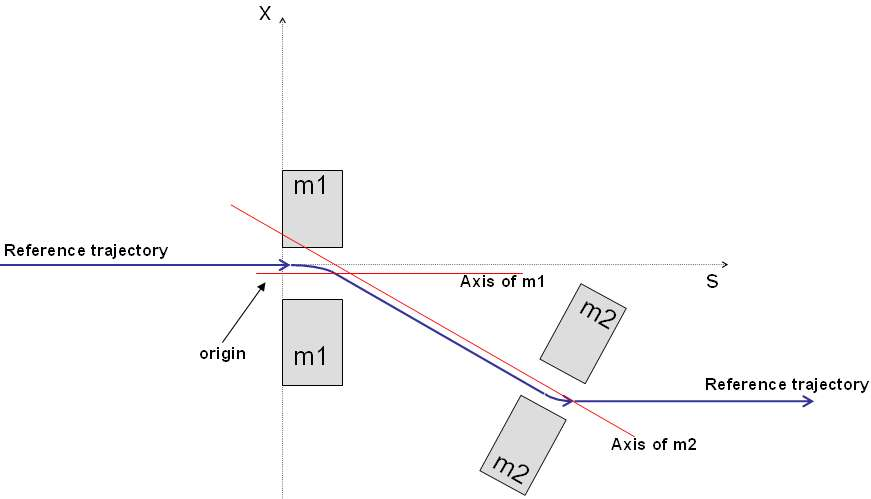
\includegraphics{offsetelem.jpg align=center width=780}
%% \\ 
%% The X\_ref(s) and Y\_ref(s) of the reference trajectory are
%% calculated via an internal call to the
%% \href{../survey/survey.html}{Survey} module. X\_offs(s) and Y\_offs(s)
%% are derived from the coefficients given in the file. The resulting  
%% \begin{verbatim}
%% X_tot(s) = X_ref(s) - X_offs(s)
%% \end{verbatim} 
%% and 
%% \begin{verbatim}
%% Y_tot(s) = Y_ref(s) - Y_offs(s)
%% \end{verbatim} 
%% are taken into account in the aperture calculations.  


\section{Aperture command example}
\label{sec:aperexample}
The aperture module needs a Twiss table to operate on. It is important
not to USE another period or sequence between the Twiss and aperture
module calls, else aperture looses its table. One can choose the ranges
for Twiss and aperture freely, they need not be the same.  

\begin{verbatim}
use, period=lhcb1;
select, flag=twiss,range=mb.a14r1.b1/mb.a17r1.b1,column=keyword,name,
parent,k0l,k1l,s,betx,bety,n1;
twiss, file=twiss.b1.data, betx=beta.ip1, bety=beta.ip1, x=+x.ip1, 
y=+y.ip1, py=+py.ip1;
plot,haxis=s,vaxis=betx,bety,colour=100;

select, flag=aperture, column=name,n1,x,dy;
aperture, range=mb.b14r1.b1/mb.a17r1.b1, spec=5.235;
plot,table=aperture,noline,vmin=0,vmax=10,haxis=s,vaxis=n1,spec,
on_elem,style=100;
\end{verbatim}

The \hyperref[sec:select]{\texttt{SELECT}} command can be  used to
choose which columns to print in the output file.   
\\ Column names: \texttt{name, n1, n1x\_m, n1y\_m, apertype, aper\_1, aper\_2,
aper\_3, aper\_4, rtol, xtol, ytol, s, betx, bety, dx, dy, x, y, on\_ap,
on\_elem, spec}  

\texttt{n1} is the maximum beam size in sigma, while n1x\_m and n1y\_m is the n1
values in si-units in the x- and y-direction.  

Note that specifying the \texttt{apertype} column automatically selects also the
\texttt{aper\_1, aper\_2, aper\_3} and \texttt{aper\_4} columns. The statement
\madxmp{
SELECT, FLAG=aperture, COLUMN=apertype;
}
is equivalent to
\madxmp{
SELECT, FLAG=aperture, COLUMN=apertype, aper\_1, aper\_2, aper\_3, aper\_4;
}

aper\_\# means for all apertypes but racetrack:
\\ aper\_1 = half width rectangle
\\ aper\_2 = half heigth rectangle
\\ aper\_3 = half horizontal axis ellipse (or radius if circle)
\\ aper\_4 = half vertical axis ellipse

For racetrack, the aperture parameters will have the same meaning as the
tolerances: 
\\ aper\_1 and xtol = horizontal displacement of radial part 
\\ aper\_2 and ytol = vertical displacement of radial part 
\\ aper\_3 and rtol = radius 
\\ aper\_4 = not used 

\texttt{ON\_ELEM} indicates whether the node is an element or a drift, and
\texttt{ON\_AP} whether it has a valid aperture. The Twiss parameters are the
interpolated values used for aperture computation.  

When one wants to plot the aperture, the \texttt{TABLE=aperture} parameter
is necessary. The normal line of hardware symbols along the top is not
compatible with the aperture table, so it is best to include
\texttt{NOLINE}. Plot instead the column \texttt{ON\_ELEM} along the
\texttt{VAXIS} to have a simple picture of the hardware. \texttt{SPEC}
can be used for giving a limit value for \texttt{n1}, to have something
to compare with on the plot. The following plot shows the \texttt{n1},
beta functions, and the hardware symbolized by \texttt{ON\_ELEM}.     

\begin{figure}[ht]  
  \centering
  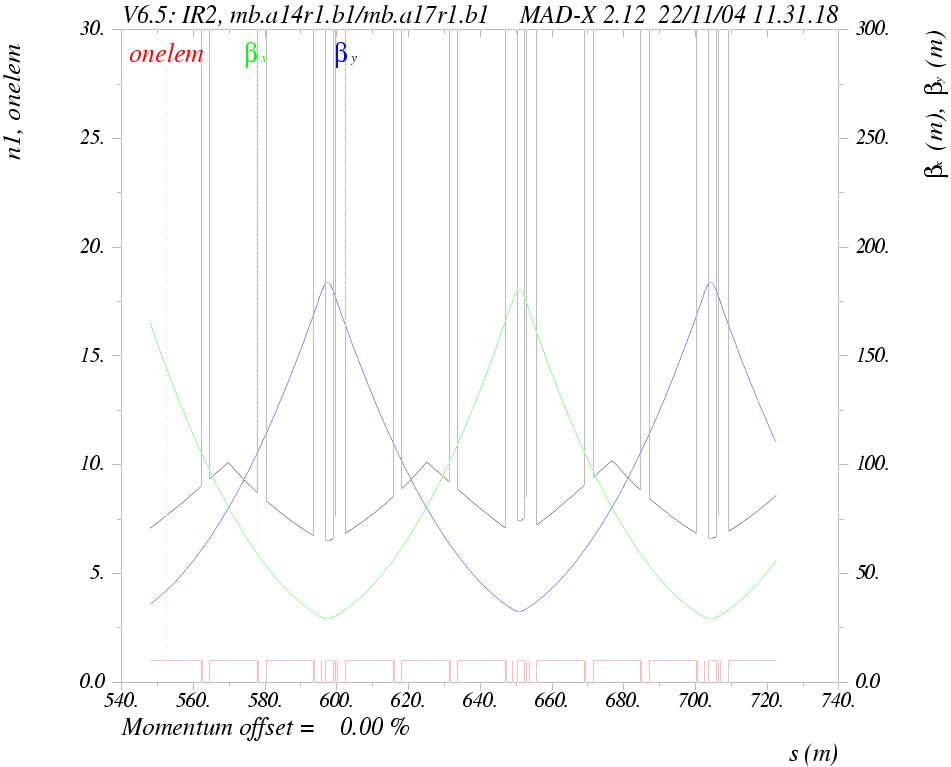
\includegraphics[width=440bp]{jpg/aperexample.jpg}
  \caption{Example of plot showing aperture limits and n1}
  \label{fig:aperexample}  
\end{figure}

% Ivar Waarum, 24.02.05  -  Mark Hayes, 19.06.02 

